\documentclass[11pt,a4paper]{article}

% ----- Page layout -----
\usepackage[a4paper,margin=2.5cm]{geometry}
\usepackage{parskip}
\usepackage{microtype}

% ----- Math -----
\usepackage{amsmath,amssymb,amsfonts}
\usepackage{mathtools}
\usepackage{siunitx}
  \sisetup{per-mode=symbol, range-units=single, range-phrase={--}}

% ----- Graphics & figures -----
\usepackage{graphicx}
\usepackage{float}
\usepackage{caption}
\captionsetup{font=small,labelfont=bf,skip=4pt}
\usepackage{subcaption}

% ----- Tables -----
\usepackage{booktabs}
\usepackage{array}
\usepackage{tabularx}
\usepackage{multirow}

% ----- Headers, hyperlinks, colors -----
\usepackage{xcolor}
\usepackage{hyperref}
\hypersetup{
  colorlinks=true,
  linkcolor=blue!60!black,
  urlcolor=blue!60!black,
  citecolor=blue!60!black
}
\usepackage{fancyhdr}
\pagestyle{fancy}
\fancyhf{}
\fancyhead[L]{\small EE4615 -- Digital IC Design II}
\fancyhead[R]{\small Group 22 -- 2-D Vernier TDC}
\fancyfoot[C]{\thepage}
\renewcommand{\headrulewidth}{0.4pt}

% ----- Custom commands -----
\newcommand{\ttau}[1]{\tau_{#1}}
\newcommand{\tlsb}{t_{0}}
\newcommand{\sumw}{\Sigma W}
\newcommand{\dt}{\Delta t}
\newcommand{\Vdd}{V_{\mathrm{DD}}}

\begin{document}

% ===================== Title page =====================
\begin{titlepage}
\centering
\vspace*{1cm}
{\large\textbf{DELFT UNIVERSITY OF TECHNOLOGY}}\\[2pt]
{\small Faculty of Electrical Engineering, Mathematics and Computer Science}\\[2cm]

\includegraphics[width=0.25\textwidth]{figures/tudelft_logo.jpeg}\\[2cm]
{\Large\textbf{A 15 ps Two-Dimensional Vernier}}\\[6pt]
{\Large\textbf{Time-to-Digital Converter in 180 nm BCD}}\\[10pt]
{\large Design report}\\[6pt]
{\large Digital IC Design II (EE4615)}\\[1.5cm]

\begin{minipage}{0.85\textwidth}
\centering\small
5-bit thermometer output, calibrated resolution \SIrange{15.0}{15.85}{\pico\second},
validated in all five process corners.\\
Schematic and Spectre simulation only; every cell hand-designed in
TSMC \SI{180}{\nano\meter} BCD.
\end{minipage}
\vfill
\rule{0.7\textwidth}{0.4pt}\\[4pt]
{\large Group 22}\\[4pt]
{\large Daniel Tyukov \quad 5714699}\\[2pt]
{\large Joris Hoogeweegen \quad 5619963}\\[4pt]
{\normalsize Delft, 15 June 2026}\\[4pt]
\rule{0.7\textwidth}{0.4pt}
\vspace{1cm}
\end{titlepage}

% ===================== Abstract =====================
\begin{abstract}
\noindent
This report presents the design and verification of a 5-bit two-dimensional
Vernier time-to-digital converter (TDC) in TSMC \SI{180}{\nano\meter} BCD.
Two delay lines with $\ttau{1}=\SI{90}{\pico\second}$ and
$\ttau{2}=\SI{75}{\pico\second}$ span a $10\times6$ comparison grid whose 31
thermometer levels each map to exactly one SR-latch arbiter, so no combining
logic is needed. The resolution $\tlsb=\ttau{1}-\ttau{2}=\SI{15}{\pico\second}$
sits well below the \SI{20}{\pico\second} specification and below the
technology gate delay. Three design decisions carry the result: fan-out-of-one
delay cells that break the \SI{97}{\pico\second} floor of conventional
fan-out-of-four sizing, characterization against a replica of the true in-grid
load of roughly twenty unit inverters, and dummy latches that equalize the
fan-out of every tap. With one fixed trim setting the converter passes all sign-off checks
in all five process corners (LSB \SIrange{13.1}{18.2}{\pico\second}, worst DNL
\num{0.90} LSB, no missing codes). Switched MOSCAP trim banks then re-center
the LSB per corner to \SIrange{15.0}{15.85}{\pico\second}, a six times tighter
spread. The core measures \SI{11.7}{\pico\joule} per conversion at a figure of
merit of \SI{0.50}{\pico\joule} per step, with a total transistor width of
\SI{1305.6}{\micro\meter}. The arbiter dead zone is below \SI{1}{\femto\second}.
A one-dimensional Vernier row built from the same cells was measured for
comparison and confirms both the loading analysis and the area advantage of the
two-dimensional architecture.
\end{abstract}

\vspace{0.5em}

\section{Introduction}
\label{sec:intro}

\subsection{Background and motivation}

A time-to-digital converter quantizes the interval between two signal edges.
In an all-digital PLL it replaces the analog phase detector and charge pump,
which made TDCs standard in digital RF synthesis; they also appear in LiDAR
and time-of-flight imaging \cite{staszewski2005, henzlerbook}. The basic flash TDC, a delay line sampled
along its taps, has a resolution floor of one gate delay. In
\SI{180}{\nano\meter} CMOS that floor is several tens of picoseconds under
realistic loading (our own loaded stage measures \SI{97}{\pico\second} at
fan-out-of-four sizing), above the \SI{20}{\pico\second} this project
requires, so a sub-gate-delay technique is mandatory.

The Vernier principle reaches below the gate delay by racing two delay lines:
the START edge propagates through stages of delay $\ttau{1}$ while the STOP
edge chases it through faster stages of delay $\ttau{2}$. The effective
resolution is the difference $\tlsb=\ttau{1}-\ttau{2}$, which can be made
arbitrarily small in principle \cite{dudek2000}. The classical one-dimensional
implementation pays for this with hardware and latency: one stage pair and one
arbiter per code, so range and resolution fight each other. Ring topologies
reuse a short line to recover range at the cost of control complexity
\cite{yu2010}; passive interpolation attacks the problem from the matching side
\cite{henzler2008}. The two-dimensional Vernier of Liscidini, Vercesi and
Castello \cite{liscidini2009, vercesi2010} instead compares \emph{every} START
tap against \emph{every} STOP tap, so a grid of $N_X+N_Y$ stages covers
$\mathcal{O}(N_X N_Y)$ distinct intervals. We chose this architecture: it
decouples range from line length and suits a course budget measured in
transistor width.

\subsection{Objectives and boundary conditions}

The EE4615 brief sets hard requirements and a design-quality trade-off
(Table~\ref{tab:spec}). Every gate must be hand-designed in TSMC
\SI{180}{\nano\meter} BCD; standard cells are not allowed. Verification is by
Spectre simulation of the schematic, no layout. The course testbench fixes the
interface: a \SI{40}{\pico\second} RESET pulse, START and STOP inputs each
driven through $3\times$ minimum inverters, and 31 thermometer outputs
$Q_{1..31}$, each loaded by the \texttt{TDC\_out} cell (two $2\times$ inverters
and \SI{1}{\femto\farad}) \cite{ee4615tb}. Robustness must be demonstrated in
the five process corners TT, SS, FF, SF and FS \cite{ee4615corner}.

\begin{table}[H]
\centering
\small
\caption{Project requirements and quality metrics.}
\label{tab:spec}
\begin{tabular}{l l}
\toprule
\textbf{Requirement} & \textbf{Value} \\
\midrule
Output & 5 bit, thermometer code $Q_{1..31}$ \\
Resolution (LSB) & better than \SI{20}{\pico\second} \\
Range & full 32-code linear range \\
Process / supply & TSMC \SI{180}{\nano\meter} BCD, \SI{1.8}{\volt} \\
Corners & TT, SS, FF, SF, FS, all must pass \\
Standard cells & none; all cells hand-designed \\
Verification & schematic + Spectre only \\
\midrule
\textbf{Quality metric} & \textbf{Definition} \\
\midrule
Linearity & DNL, INL per corner \\
Energy & average energy per conversion \\
Area & total transistor width $\sumw$ \\
Figure of merit & energy per conversion step \\
\bottomrule
\end{tabular}
\end{table}

\subsection{Contributions and report structure}

The delivered converter reaches a calibrated resolution of
\SIrange{15.0}{15.85}{\pico\second} in all five corners with no missing codes.
Beyond meeting the specification, the project contributes three results that we
believe generalize: a quantified demonstration that fan-out-of-four sizing
cannot reach the required stage delays in this technology, a replica-load
sizing method for Vernier grids in which each tap drives on the order of twenty
unit gates, and a measured one-dimensional versus two-dimensional comparison
built from identical cells that isolates the architectural benefit from the
circuit design.

Section~\ref{sec:arch} develops the architecture and the operating point.
Section~\ref{sec:circuits} documents every cell with its transistor sizes.
Section~\ref{sec:method} describes the design iterations and the verification
setup. Section~\ref{sec:results} reports the corner, calibration, energy,
metastability and comparison results, and Section~\ref{sec:conclusion}
concludes.

\section{Architecture}
\label{sec:arch}

\subsection{From one to two dimensions}

In a 1-D Vernier TDC the STOP edge gains $\tlsb=\ttau{1}-\ttau{2}$ on the START
edge at every stage, and an arbiter at each stage records whether STOP has
caught up. Resolving the 31 thermometer levels therefore takes 31 stages in
each line and 31 arbiters, and the conversion latency grows with the full
$31\,\ttau{1}$. The
2-D Vernier \cite{vercesi2010} generalizes the race: with START applied to a
line of $N_X$ stages of delay $\ttau{1}$ and STOP to a line of $N_Y$ stages of
delay $\ttau{2}$, an arbiter at grid position $(i,j)$ compares the edge leaving
START stage $i$ with the edge leaving STOP stage $j$ and fires when
\begin{equation}
  \dt > i\,\ttau{1} - j\,\ttau{2}.
  \label{eq:cell}
\end{equation}
Each cell therefore measures its own threshold, and $N_X+N_Y$ stages yield up
to $N_X N_Y$ distinct thresholds. Range no longer dictates line length.

\subsection{Bijective level mapping at $k=6$}

We restrict the design space to the family
$\ttau{1}=k\,\tlsb$, $\ttau{2}=(k-1)\,\tlsb$. In this family the threshold of
cell $(i,j)$ equals $(ik - j(k-1))\,\tlsb$, an exact integer multiple of the
LSB, and the mapping from thermometer level $m$ to grid cell is bijective
\cite{vercesi2010}:
\begin{equation}
  y_m = \bigl((m-1) \bmod k\bigr) + 1,
  \qquad
  x_m = \frac{m + (k-1)\,y_m}{k},
  \qquad m = 1,\dots,31.
  \label{eq:mapping}
\end{equation}
Level $m$ is exactly one SR latch, wired straight to output $Q_m$. No OR tree
or encoder sits between arbiter and output, so combining-logic skew cannot
corrupt the code. For $k=6$ the mapping spans $x_m \le 10$ and $y_m \le 6$: a
$10\times6$ logical grid, 10 START stages and 6 STOP stages for all 31 levels.

The operating point follows from two constraints. The LSB must clear the
\SI{20}{\pico\second} specification with margin for corner spread, which sets
$\tlsb=\SI{15}{\pico\second}$. The stage delays must stay inside the window
that the delay cell can actually produce under its in-grid load
(Section~\ref{sec:method}), which selects $k=6$:
$\ttau{1}=\SI{90}{\pico\second}$ and $\ttau{2}=\SI{75}{\pico\second}$. Smaller
$k$ would require $\ttau{2}$ below the achievable minimum; larger $k$ would
lengthen both lines and add area without improving resolution.

\begin{figure}[H]
\centering
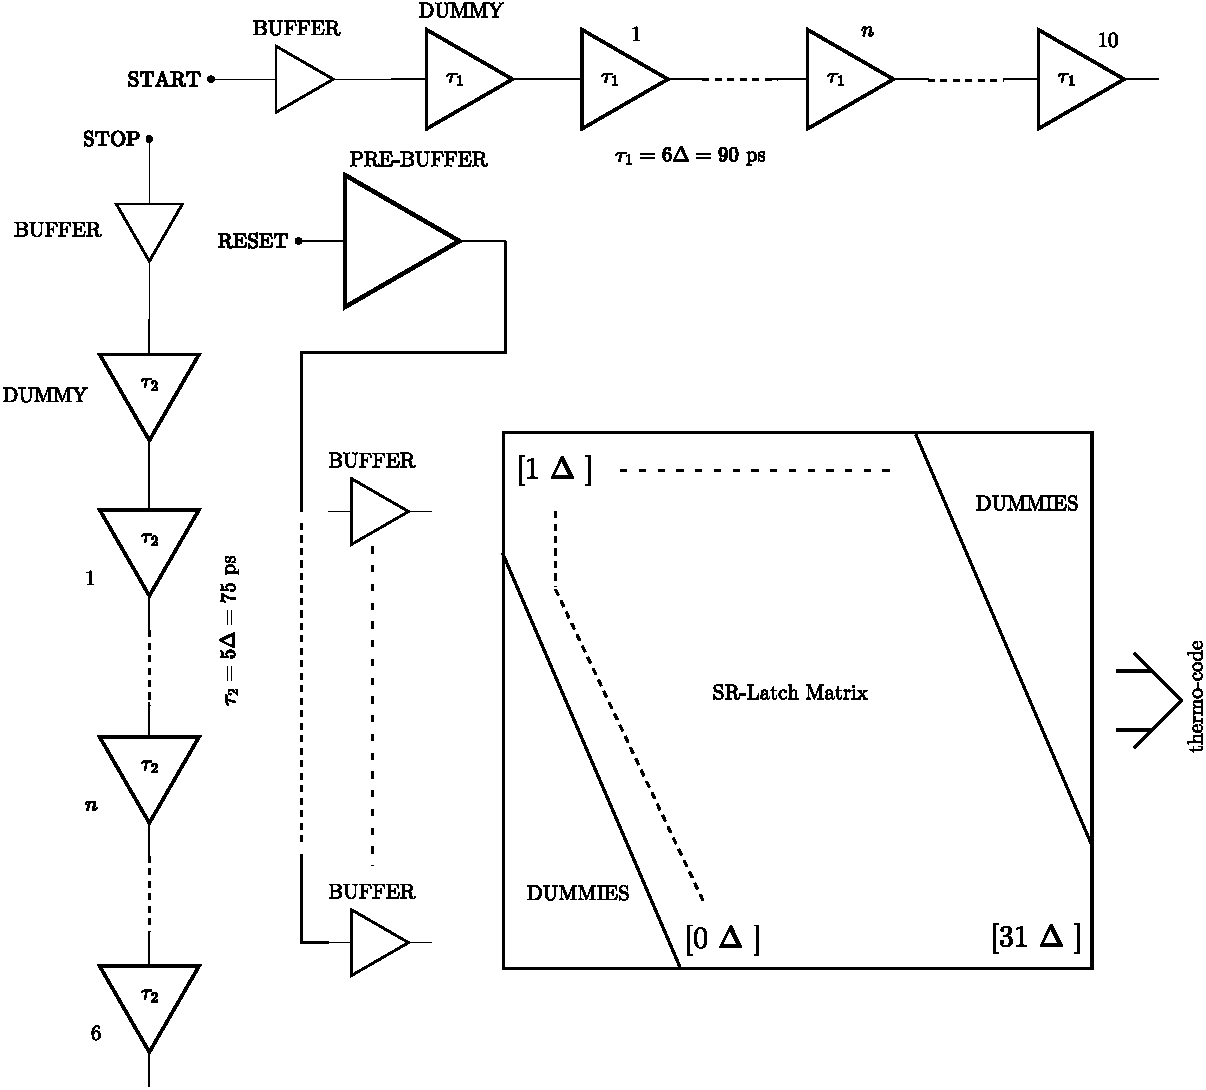
\includegraphics[width=0.82\textwidth]{figures/overview.pdf}
\caption{Top level of the converter. The START line (10 stages of $\ttau{1}$,
top) and the STOP line (6 stages of $\ttau{2}$, left) feed the SR-latch matrix.
The 31 active latches sit on the bijective map of Eq.~\eqref{eq:mapping};
dummy latches pad every tap to identical fan-out. Buffer trees distribute
START, STOP and the \SI{40}{\pico\second} RESET. The thermometer code is read
directly from the latch outputs.}
\label{fig:overview}
\end{figure}

\subsection{Fan-out equalization and reset}

Equation~\eqref{eq:cell} only holds if every stage of a line contributes the
same delay, and stage delay depends on load. In the raw $10\times6$ grid the
taps drive between one and ten latches, which would modulate the stage delays
along the line and corrupt the thresholds. We therefore pad the array with 29
dummy latches to a physically symmetric $10\times6$ arrangement: 31 active
plus 29 dummy latches give every START tap and every STOP tap the same fan-out
of ten latch inputs. The dummies are electrically identical to active latches;
only their outputs are unused. The same uniformity argument adds one extra
delay cell at the head of each line (11 and 7 cells in total), so that the
first logical stage sees the same driver as all others.

Each latch carries an asynchronous clear input. The \SI{40}{\pico\second}
RESET pulse from the testbench, widened through its own buffer tree, clears
all 60 latches before each conversion so that every conversion starts from
$Q_m=0$.

\section{Circuit design}
\label{sec:circuits}

All cells were designed at transistor level in the \texttt{vernier2d} library
using the \SI{2}{\volt} devices of the \texttt{tsmc18} library
(\texttt{nmos2v}/\texttt{pmos2v}, Spectre models \texttt{nch}/\texttt{pch}) at
the minimum channel length $L=\SI{180}{\nano\meter}$.
The unit inverter used throughout is $W_p/W_n = \SI{440}{\nano\meter}/\SI{220}{\nano\meter}$;
larger drivers are built as parallel fingers (multiples) of this unit.
Table~\ref{tab:cells} summarizes the cell inventory; the per-cell width budget
is given in Appendix~\ref{app:sigmaw}.

\begin{table}[H]
\centering
\small
\caption{Cell inventory of the TDC core with device sizing. All lengths
\SI{180}{\nano\meter} except the MOSCAPs (\SI{250}{\nano\meter}).}
\label{tab:cells}
\begin{tabularx}{\textwidth}{l c X}
\toprule
\textbf{Cell} & \textbf{Count} & \textbf{Contents and sizing} \\
\midrule
\texttt{delay\_tau1} & 11 &
FO=1 inverter pair ($10\times$ input, $10\times$ driver, unit
$440/\SI{220}{\nano\meter}$); MOSCAP's for trimming: three TG-switched trim banks of
$2/20/21$ fingers and one fixed TG-MOSCAP ($7/18$ fingers) connection to ensure $\tau_1=\tau_2+15\mathrm{ps}$. \\
\texttt{delay\_tau2} & 7 &
identical active devices as \texttt{delay\_tau1}; lighter trim banks of
$2/14/18$ fingers. \\
\texttt{srlatch} & 60 &
13 transistors: two 2-input NANDs (all devices
$440/\SI{180}{\nano\meter}$), asynchronous-reset NMOS
($2.0/\SI{0.18}{\micro\meter}$), two unit-inverter output buffers. \\
\texttt{nand} & (in latch) &
two series NMOS, two parallel PMOS, all $440/\SI{180}{\nano\meter}$. \\
\texttt{Inv\_10x/20x/40x/80x} & trees &
input and reset distribution buffers, parallel-finger multiples of the unit
inverter. \\
\bottomrule
\end{tabularx}
\end{table}

\subsection{Delay stage}
\label{sec:delaycell}

\begin{figure}[H]
\centering
\begin{subfigure}[t]{0.58\textwidth}
  \centering
  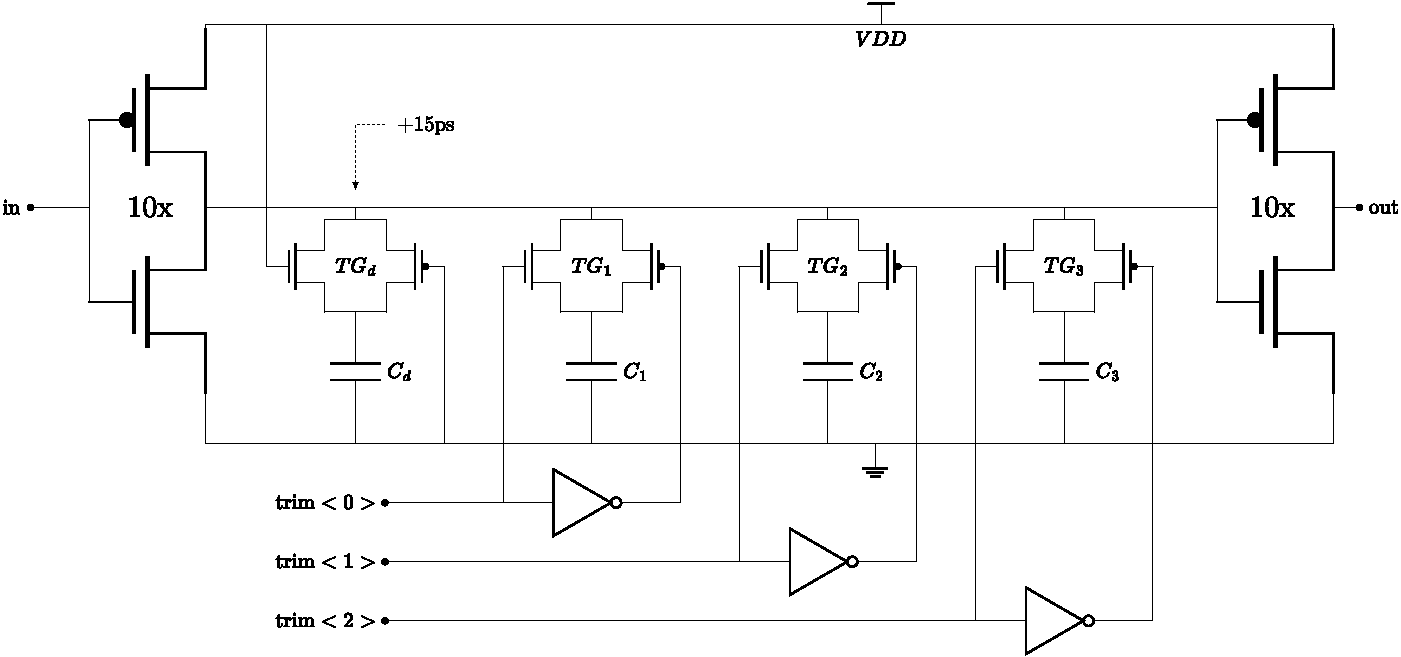
\includegraphics[width=\textwidth]{figures/delay_tau1.pdf}
  \caption{\texttt{delay\_tau1} (START line, \SI{90}{\pico\second}).}
  \label{fig:tau1}
\end{subfigure}\hfill
\begin{subfigure}[t]{0.40\textwidth}
  \centering
  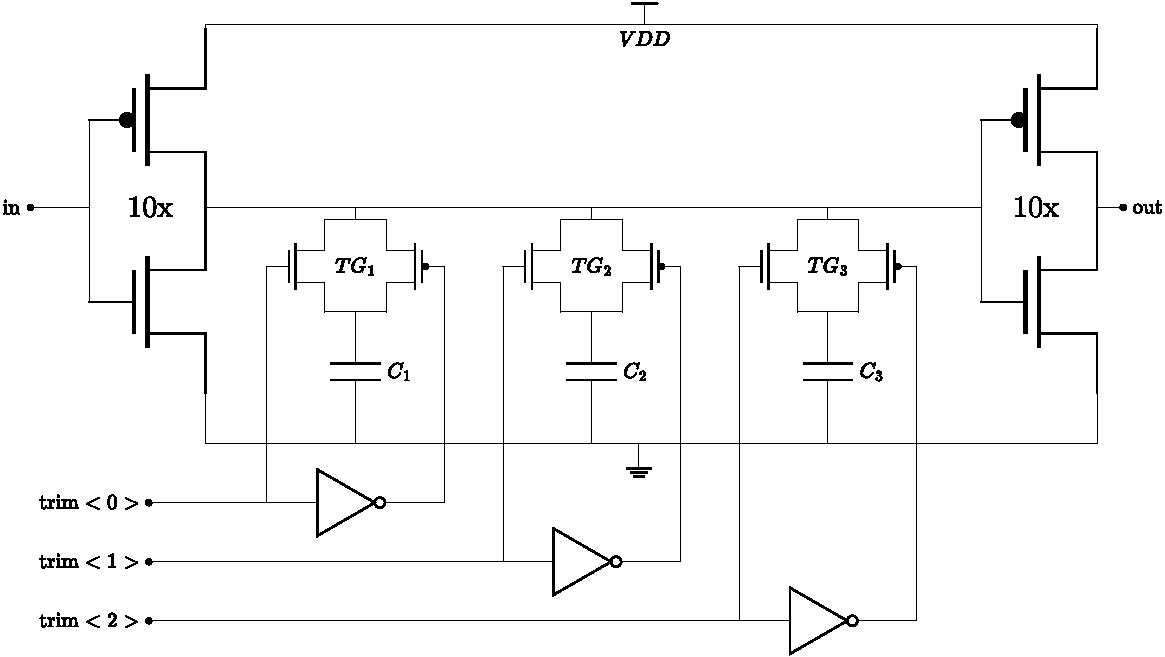
\includegraphics[width=\textwidth]{figures/delay_tau2.pdf}
  \caption{\texttt{delay\_tau2} (STOP line, \SI{75}{\pico\second}).}
  \label{fig:tau2}
\end{subfigure}
\caption{Delay stages. An FO=1 inverter pair drives the next stage; the
internal node carries one fixed MOSCAP behind an always-on access transistor
plus three transmission-gate-switched MOSCAP banks controlled by
\texttt{trim<0:2>}. The two cells differ only in bank sizes.}
\label{fig:delaycells}
\end{figure}

The delay stage is a two-inverter buffer whose internal node is loaded
capacitively (Fig.~\ref{fig:delaycells}). Two choices define it.

\textbf{Fan-out of one.} Conventional FO=4 sizing minimizes the delay of a
logic path, but here delay is the product, not the cost. With FO=4 the
intrinsic delay of the internal node pins the minimum achievable stage delay at
\SI{97}{\pico\second} in this technology, which already exceeds the required
$\ttau{2}$. Equal input and driver sizing ($10\times$ and $10\times$ unit
fingers) reduces the internal-node capacitance and opens a usable window of
\SIrange{74}{147}{\pico\second} under the true grid load.

\textbf{Capacitive tuning, identical actives.} Both lines use the same active
devices; only the capacitance on the internal node differs. The fixed MOSCAP
($18\times$ fingers, $L=\SI{250}{\nano\meter}$) sets the nominal delay, and
three banks ($2/20/21$ fingers on the $\ttau{1}$ cell,
$2/14/18$ on the $\ttau{2}$ cell) are switched in or out through transmission
gates by the static \texttt{trim<0:2>} inputs. Because both delays have the same $10\times, FO=1$ sizing, $\ttau{1}$ and $\ttau{2}$ track
each other over process and temperature, which is what keeps their difference,
the LSB, stable. At the tuned typical-corner point the lines measure
$\ttau{1}=\SI{90.5}{\pico\second}$ and $\ttau{2}=\SI{75.4}{\pico\second}$.

\subsection{Arbiter}
\label{sec:arbiter}

\begin{figure}[H]
\centering
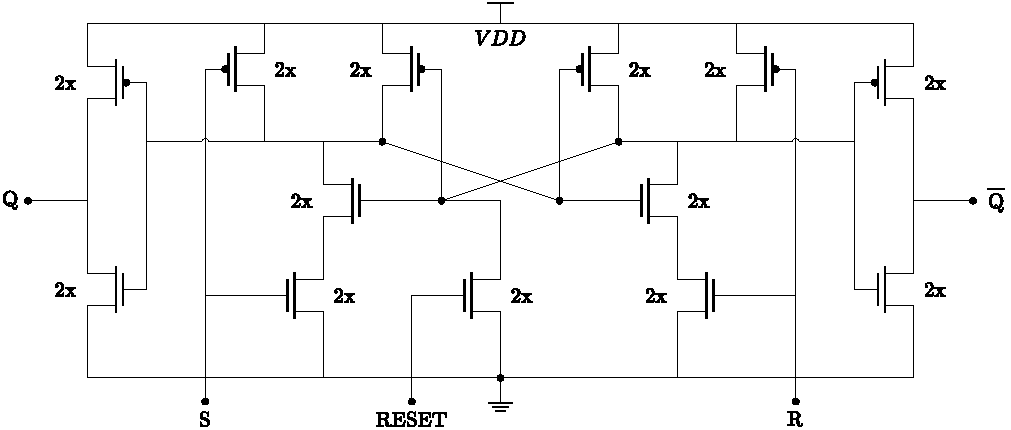
\includegraphics[width=0.8\textwidth]{figures/srlatch.pdf}
\caption{SR-latch arbiter (\texttt{vernier2d/srlatch}). Two cross-coupled
NANDs ($440/\SI{180}{\nano\meter}$ throughout), an asynchronous-reset NMOS on
the internal node, and two unit-inverter output buffers. S and R are active
high; the first rising edge wins.}
\label{fig:srlatch}
\end{figure}

The arbiter decides, at each grid node, which edge arrived first. We use a
cross-coupled NAND SR latch with buffered outputs (Fig.~\ref{fig:srlatch}),
13 transistors in total. Both NAND outputs idle high; the first rising input
flips the latch and positive feedback locks the decision. Three properties
motivated the choice over a D flip-flop. The cell is small, which matters at
60 instances. The S and R paths are electrically symmetric with equal NMOS and
PMOS widths, which is what keeps the arbitration offset at the femtosecond
level measured in Section~\ref{sec:meta}. And reset costs a single NMOS
($2.0/\SI{0.18}{\micro\meter}$) that pulls one internal node during the
\SI{40}{\pico\second} RESET pulse, defining $Q=0$ before every conversion.

\subsection{Core assembly}

\begin{figure}[H]
\centering
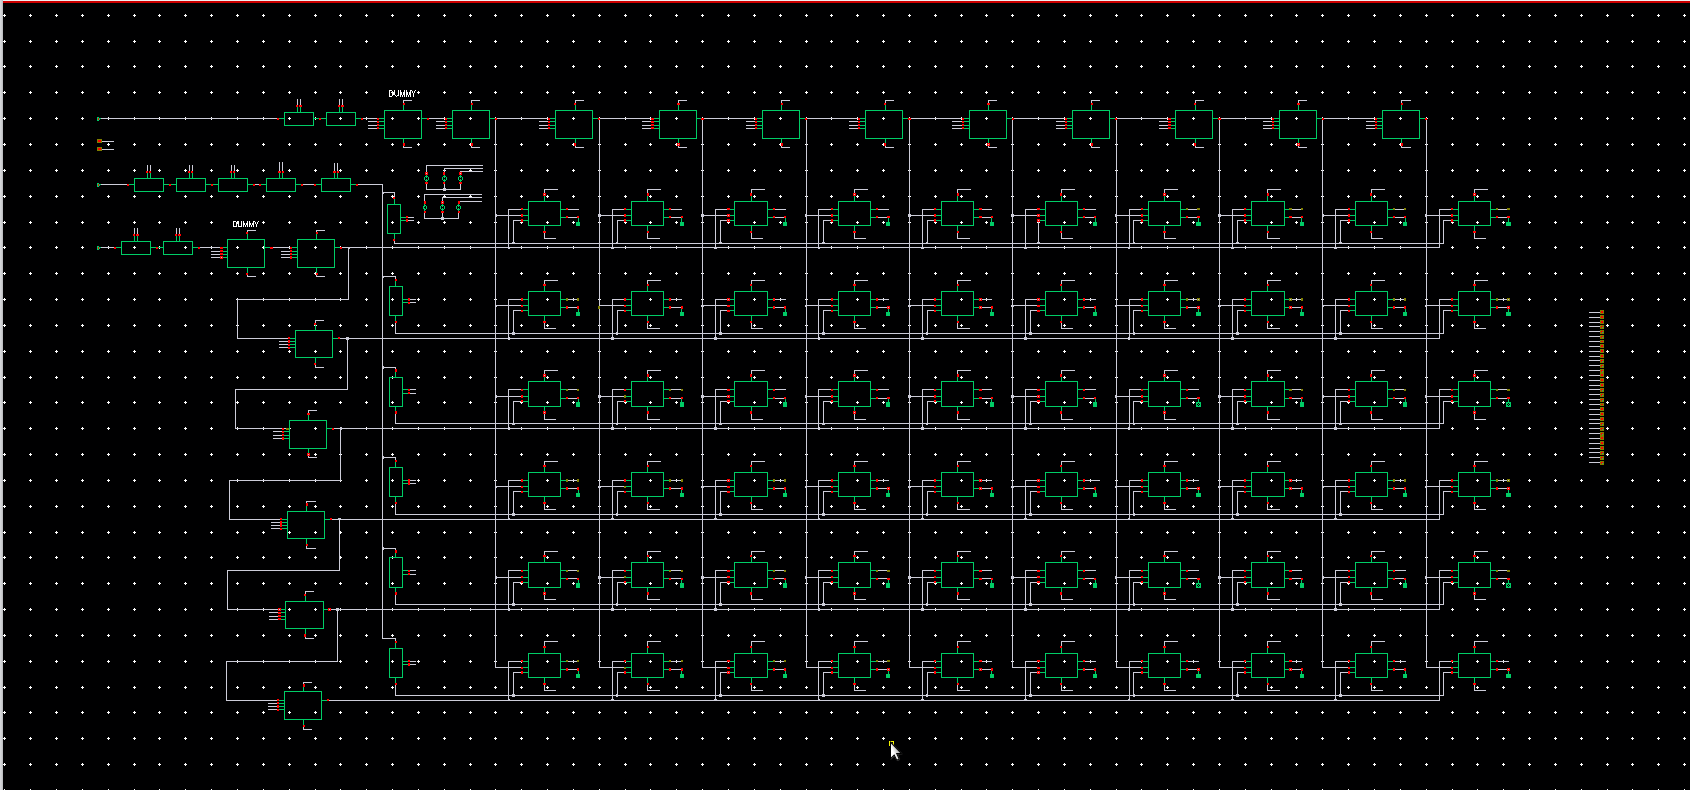
\includegraphics[width=0.95\textwidth]{figures/tdc_core_cadence.png}
\caption{\texttt{vernier2d/tdc\_core} as entered in Cadence Virtuoso: START
line across the top, STOP line down the left, and the $10\times6$ padded
latch matrix. The core contains 1120 active devices.}
\label{fig:core}
\end{figure}

The core (Fig.~\ref{fig:core}) instantiates 11 \texttt{delay\_tau1} and 7
\texttt{delay\_tau2} stages, 60 latches and the input buffer trees, and exposes
the course-mandated pins (RESET, START, STOP, $\Vdd$, GND, $Q_{1..31}$). The
six trim lines enter as static gate biases, standing in for configuration
bits. The total transistor width is $\sumw=\SI{1305.6}{\micro\meter}$:
\SI{1078.3}{\micro\meter} of active devices (1120 transistors) and
\SI{227.3}{\micro\meter} of MOSCAP (65 devices). The width budget is dominated
by the \texttt{delay\_tau1} drivers (\SI{451}{\micro\meter}) and the latch
NANDs (\SI{211}{\micro\meter}); the full breakdown is in
Appendix~\ref{app:sigmaw}.

\section{Design methodology and verification setup}
\label{sec:method}

\subsection{Sizing against the real load}
\label{sec:loading}

The decisive step of the design was recognizing what a delay stage actually
drives inside the grid. A $\ttau{2}$ tap feeds the latch inputs of an entire
row, a $\ttau{1}$ tap those of an entire column, and both feed the next delay
stage, whose input capacitance scales with the stage sizing itself. After
fan-out equalization the equivalent load is about twenty unit-inverter inputs
per tap.

Stage sizing derived from a standalone sweep with an idealized load predicted
$\tlsb=\SI{16.6}{\pico\second}$; the same cells assembled into a row with raw
tap loading measured \SI{28.6}{\pico\second} (Section~\ref{sec:1dvs2d}),
nearly a factor of two lost to loading. All final sizing was therefore done
against a replica load of ten latch inputs plus one downstream stage, swept
in the slowest corner (SS) so that the slow line stays reachable everywhere.
The same analysis moved the architecture itself: an earlier $k=4$ operating
point ($\ttau{1}/\ttau{2}=60/\SI{45}{\pico\second}$) required stage delays
below the achievable window and was abandoned in favor of $k=6$.

\subsection{Per-corner trimming}
\label{sec:calmethod}

Process corners shift both line delays together, but not perfectly, so $\tlsb$
breathes with the corner. The MOSCAP banks of Section~\ref{sec:delaycell}
absorb this. All 64 on/off combinations of the six bank gates were simulated
per corner, measuring $\ttau{1}$ and $\ttau{2}$ directly on the tap nets; the
configuration with $\tlsb$ closest to \SI{15}{\pico\second} was selected and
validated end-to-end with a full staircase sweep (Appendix~\ref{app:trim}).
Trimming changes gate voltages only, so the transistor inventory and $\sumw$
are identical in every corner.

\subsection{Testbench and measurement method}
\label{sec:testbench}

All system-level results come from the unmodified course testbench
\texttt{TB\_TDC} \cite{ee4615tb}: stimulus generation in \texttt{TDC\_in},
the DUT wrapper, and \texttt{TDC\_out} loading every thermometer output with
two $2\times$ inverters and \SI{1}{\femto\farad}. The DUT receives its supply
through a dedicated rail with a series ammeter, separate from the stimulus
rail, so the measured energy, $E=\Vdd\int |i|\,dt$ over each
\SI{5}{\nano\second} conversion window, contains only the converter.

OCEAN automates the characterization. Per corner, the input delay is swept in
\SI{1.5}{\pico\second} steps (one tenth of the LSB) across the full range,
and the scripts extract the LSB (mean step width), DNL, INL, offset, energy,
ENOB and the sign-off checks: no missing codes, monotonicity, and an intact
thermometer code at every point. The course script reports INL as the
half-range value $(\mathrm{INL}_{\max}-\mathrm{INL}_{\min})/2$, while the
plots show the endpoint-referenced per-code curve; we quote the course
convention for sign-off and state both where they differ.

\section{Results}
\label{sec:results}

All results are Spectre simulations of the schematic at \SI{27}{\celsius} and
$\Vdd=\SI{1.8}{\volt}$ through the course testbench, in the five corners TT,
SS, FF, SF and FS.

\subsection{Transfer and resolution across corners}
\label{sec:corners}

Figure~\ref{fig:staircase} shows the measured transfer with one fixed trim
configuration (the trimmed TT setting) in all five corners; Table~\ref{tab:corners}
lists the extracted metrics. Every corner produces a monotonic 31-step
staircase with an intact thermometer code, and every corner passes the
\SI{20}{\pico\second} requirement, with the slowest corner (SS,
\SI{18.2}{\pico\second}) closest to the limit. The skewed corners SF and FS
barely differ from TT because opposite N and P shifts largely cancel in an
inverter pair. The input-referred offset stays between $-7$ and
\SI{-24}{\pico\second}, constant per corner: a code offset, not a linearity
error.

\begin{figure}[htb]
\centering
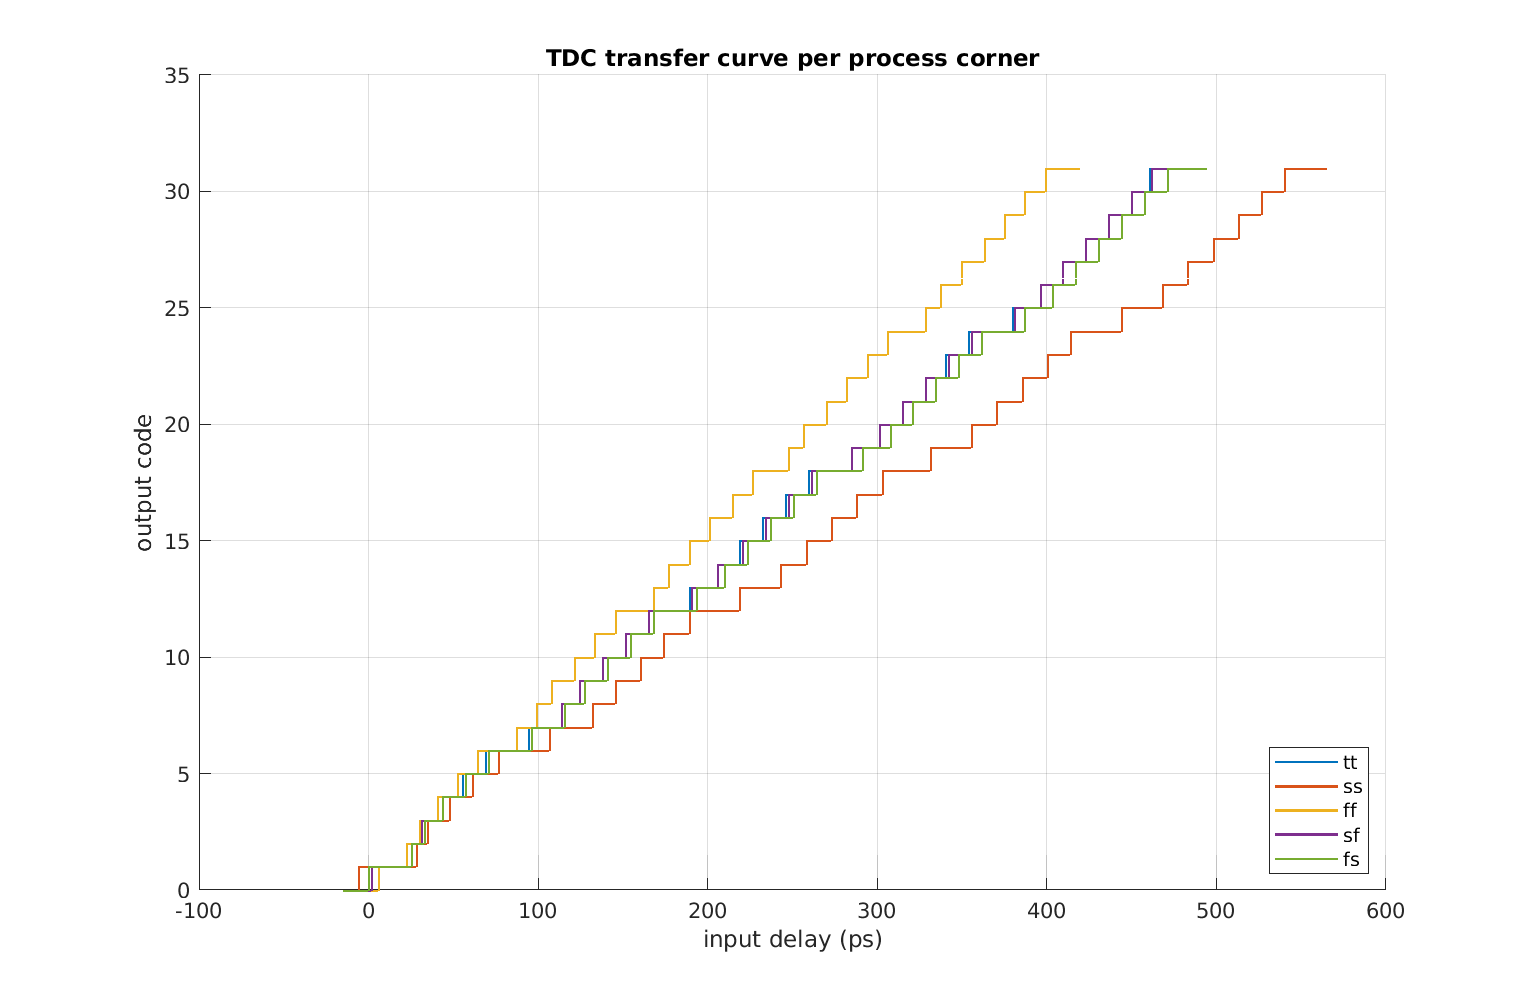
\includegraphics[width=0.72\textwidth]{figures/staircase_all_corners.png}
\caption{TDC transfer per corner, fixed trim configuration. All corners are
monotonic and reach code 31; the slope spreads with corner speed.}
\label{fig:staircase}
\end{figure}

\begin{table}[H]
\centering
\small
\caption{Corner results with one fixed trim configuration. INL is the course
half-range convention; energy and FoM from the supply-ammeter measurement.
Every corner passes all sign-off checks (no missing codes, monotonic,
LSB below \SI{20}{\pico\second}).}
\label{tab:corners}
\begin{tabular}{l S[table-format=2.2] S[table-format=1.2] S[table-format=1.2] S[table-format=-2.1] S[table-format=2.2] S[table-format=1.2] S[table-format=1.2]}
\toprule
\textbf{Corner} & {\textbf{LSB}} & {\textbf{DNL$_{\max}$}} &
{\textbf{INL}} & {\textbf{Offset}} &
{\textbf{E/conv}} & {\textbf{ENOB}} & {\textbf{FoM}} \\
 & {(\si{\pico\second})} & {(LSB)} & {(LSB)} & {(\si{\pico\second})} &
{(\si{\pico\joule})} & {(bit)} & {(\si{\pico\joule}/step)} \\
\midrule
TT & 15.35 & 0.66 & 0.65 & -15.4 & 11.67 & 4.54 & 0.50 \\
SS & 18.20 & 0.90 & 0.76 & -24.2 & 10.76 & 4.39 & 0.51 \\
FF & 13.10 & 0.72 & 0.58 & -7.1  & 12.84 & 4.58 & 0.54 \\
SF & 15.35 & 0.66 & 0.61 & -13.9 & 11.96 & 4.57 & 0.50 \\
FS & 15.70 & 0.72 & 0.61 & -15.7 & 11.38 & 4.56 & 0.48 \\
\bottomrule
\end{tabular}
\end{table}

\subsection{Linearity}
\label{sec:linearity}

\begin{figure}[htb]
\centering
\begin{subfigure}[t]{0.49\textwidth}
  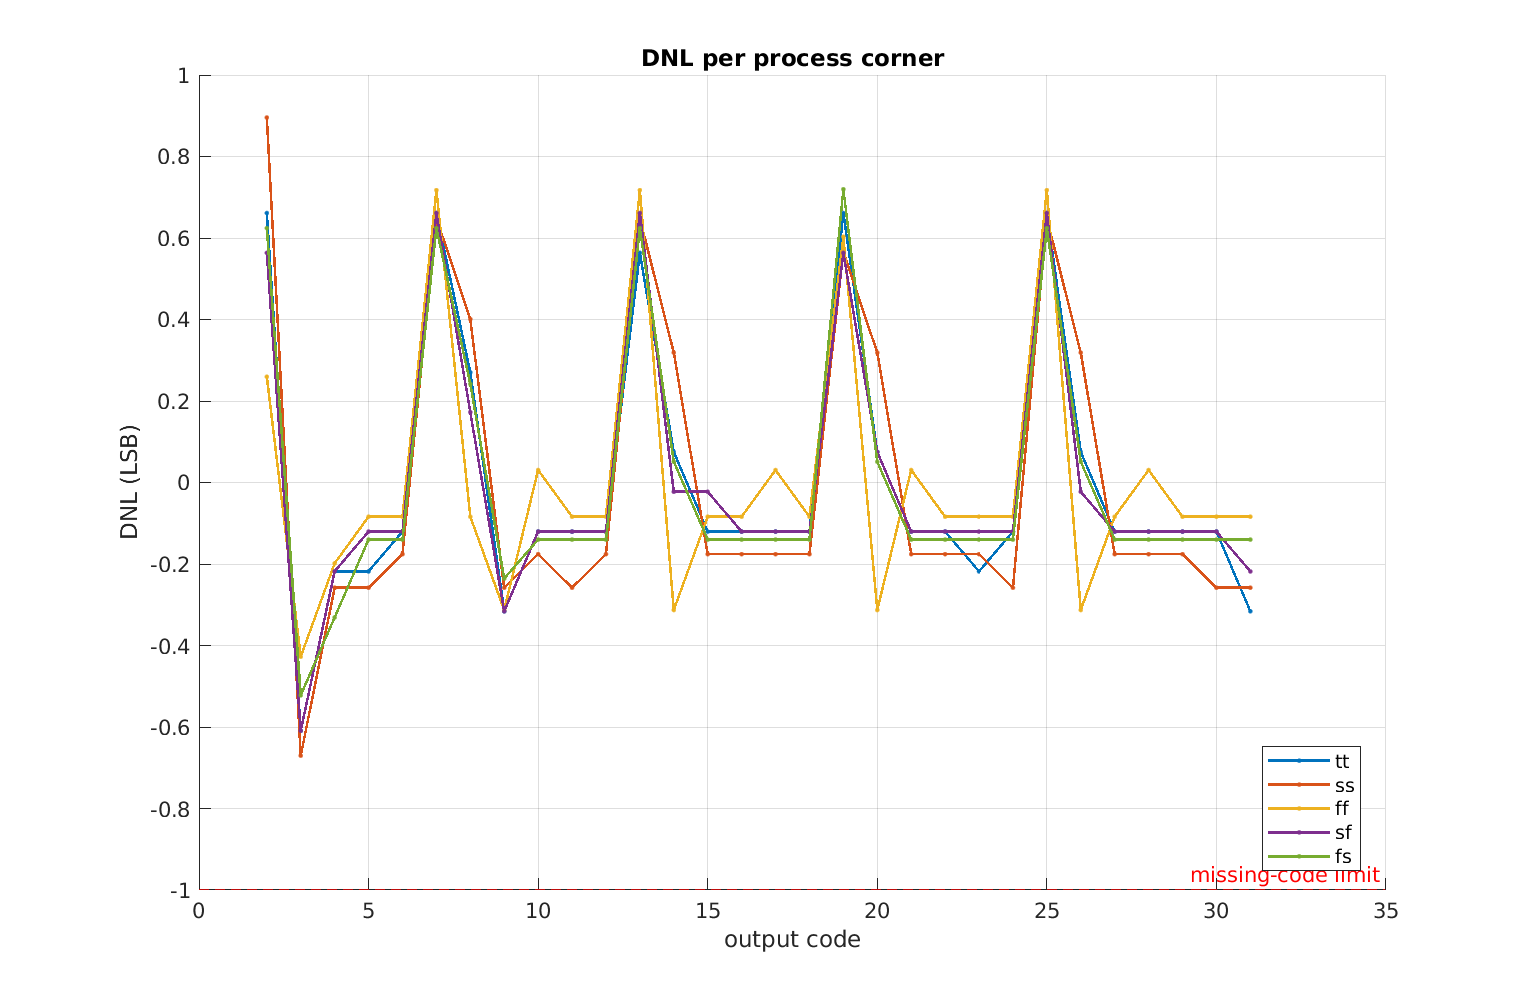
\includegraphics[width=\textwidth]{figures/dnl_per_corner.png}
  \caption{DNL per corner.}
  \label{fig:dnl}
\end{subfigure}\hfill
\begin{subfigure}[t]{0.49\textwidth}
  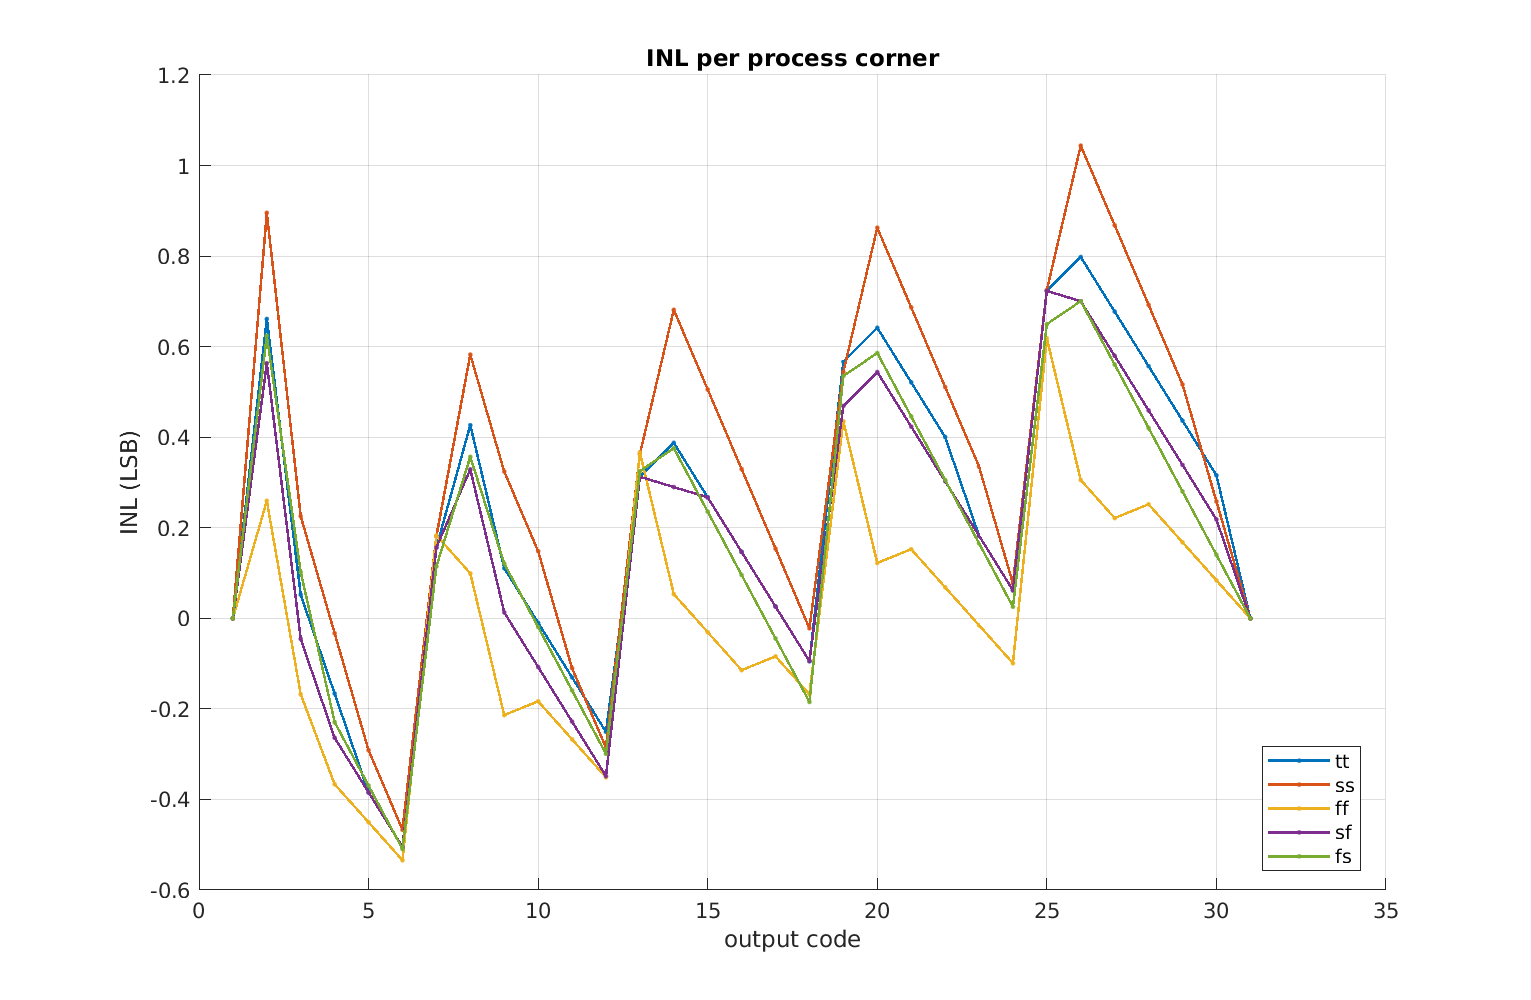
\includegraphics[width=\textwidth]{figures/inl_per_corner.png}
  \caption{INL per corner (endpoint convention).}
  \label{fig:inl}
\end{subfigure}
\caption{Linearity with fixed trim. The period-6 sawtooth marks the column-wrap
boundaries of the $k=6$ mapping and repeats identically in every corner.}
\label{fig:linearity}
\end{figure}

Worst-case DNL is \num{0.90} LSB (SS), well clear of the $-1$ LSB missing-code
limit; no corner loses a code (Fig.~\ref{fig:linearity}). Switching from the
half-range convention of Table~\ref{tab:corners} to the per-code endpoint
curve of Fig.~\ref{fig:inl}, the worst endpoint INL is \num{1.04} LSB (SS);
all other corners stay at or below \num{0.80}. The dominant DNL feature is a
sawtooth with period 6, peaking at \numrange{0.6}{0.7} LSB at codes 7, 13, 19
and 25: the column-wrap boundaries of the mapping in Eq.~\eqref{eq:mapping}.
The pattern is identical in every corner, so it is architectural rather than
mismatch-driven, and trimming cannot remove it
(Section~\ref{sec:calibration}). A targeted capacitive correction at the wrap
codes is listed as future work.

\subsection{Per-corner trimming}
\label{sec:calibration}

\begin{figure}[htb]
\centering
\begin{subfigure}[t]{0.49\textwidth}
  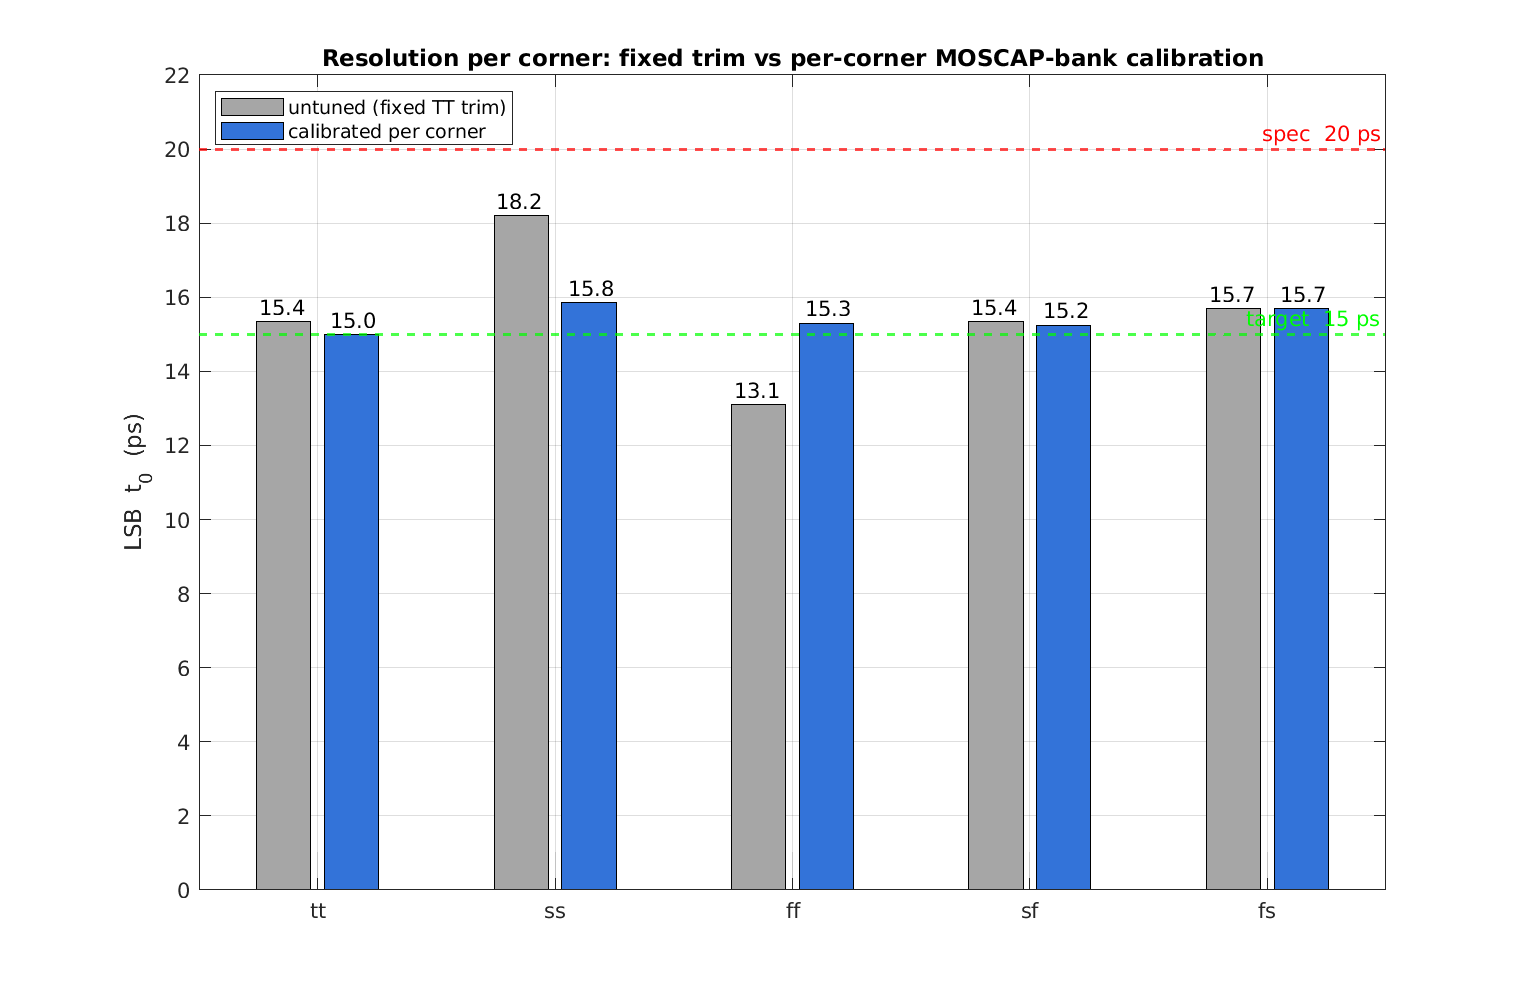
\includegraphics[width=\textwidth]{figures/lsb_tuned_vs_untuned.png}
  \caption{LSB per corner, fixed trim vs per-corner trim.}
  \label{fig:lsbtuned}
\end{subfigure}\hfill
\begin{subfigure}[t]{0.49\textwidth}
  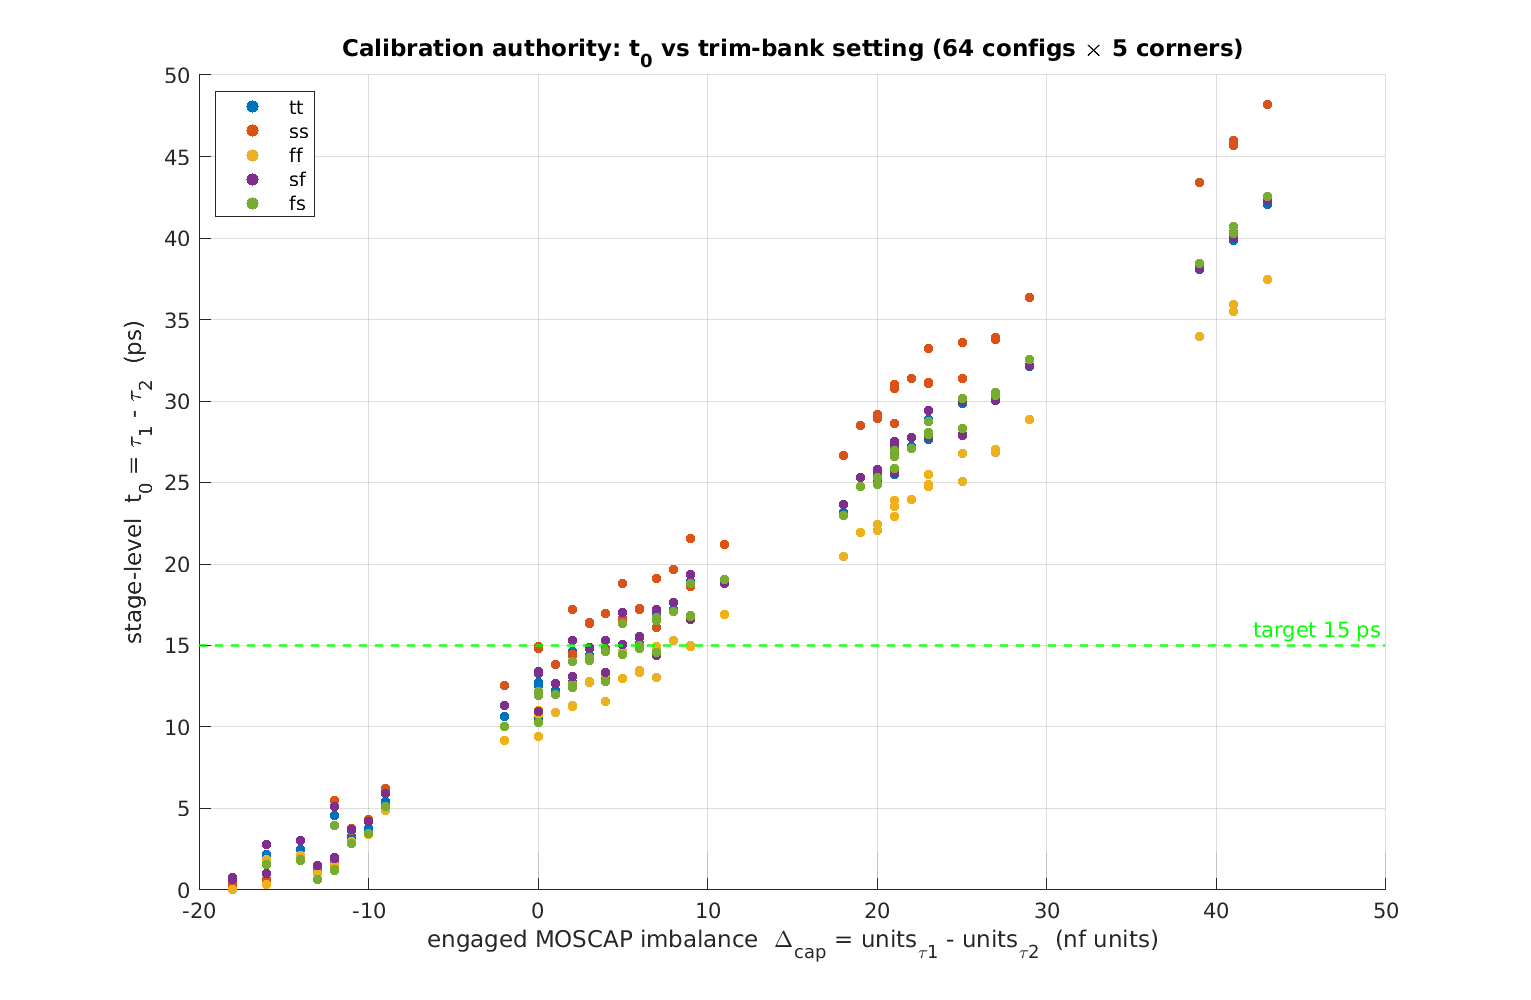
\includegraphics[width=\textwidth]{figures/calibration_range.png}
  \caption{Trim authority: stage-level $\tlsb$ vs engaged capacitance
  imbalance, all 64 configurations in 5 corners.}
  \label{fig:calrange}
\end{subfigure}
\caption{MOSCAP-bank trimming. Every corner re-centers to the
\SI{15}{\pico\second} target; the banks command roughly
\SIrange{0}{48}{\pico\second}, far more authority than the corners require.}
\label{fig:calfigs}
\end{figure}

Applying the per-corner trim codes of Appendix~\ref{app:trim} re-centers the
LSB to \SIrange{15.0}{15.85}{\pico\second}: the corner spread tightens from
\SI{5.10}{\pico\second} to \SI{0.85}{\pico\second}, six times, and the
worst-case margin to the specification grows from \num{1.8} to
\SI{4.15}{\pico\second} (Fig.~\ref{fig:lsbtuned}). DNL and INL barely move
(worst trimmed INL \num{0.74} LSB), consistent with the architectural origin
of the wrap pattern. All sign-off checks still pass in every corner.

\subsection{Energy, power and figure of merit}
\label{sec:energy}

\begin{figure}[htb]
\centering
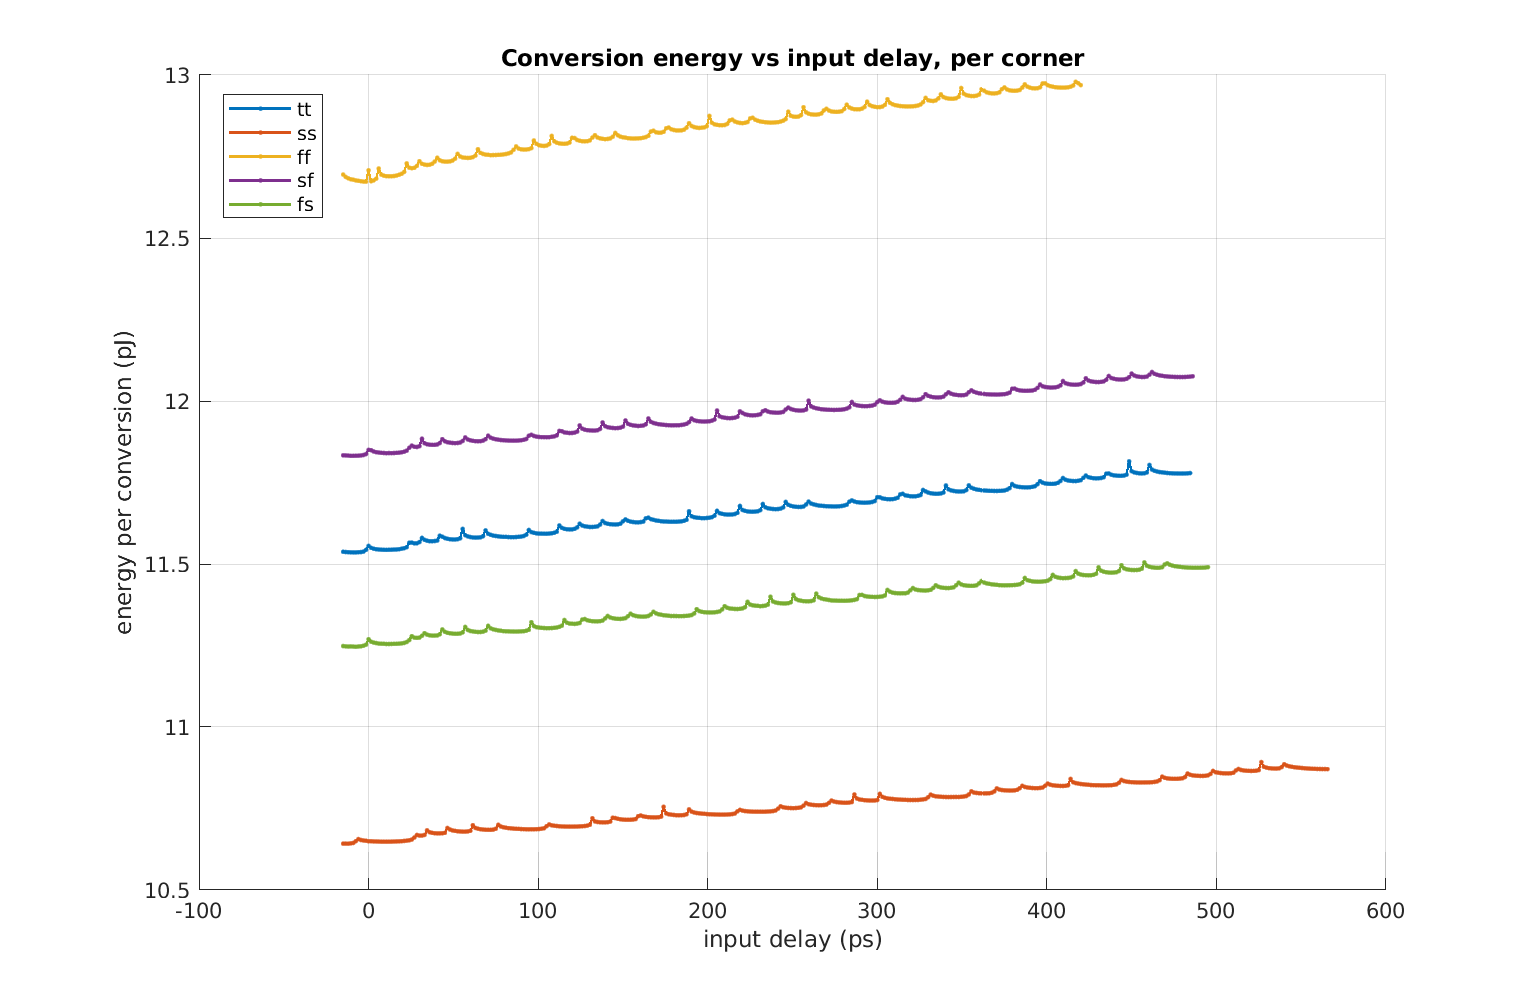
\includegraphics[width=0.62\textwidth]{figures/power_vs_delay.png}
\caption{Energy per conversion vs input delay, per corner. The band is nearly
flat; energy tracks corner speed.}
\label{fig:energy}
\end{figure}

Energy per conversion sits in a flat \SIrange{10.6}{13.0}{\pico\joule} band
across input delay and corner (Fig.~\ref{fig:energy}), ordered by corner speed
(SS lowest, FF highest). With the \SI{5}{\nano\second} conversion window of
the testbench this corresponds to an average power of
\SIrange{2.15}{2.57}{\milli\watt}. Table~\ref{tab:fom} reports both figure-of-merit
conventions: the specification's $P/\tlsb$ and the course script's
$E/2^{\mathrm{ENOB}}$. The dynamic range, $31\times\mathrm{LSB}$, spans
\SIrange{406}{564}{\pico\second} depending on the corner, with a
quantization-limited single-shot precision $\mathrm{LSB}/\sqrt{12}$ of
\SIrange{3.8}{5.3}{\pico\second}.

\begin{table}[H]
\centering
\small
\caption{Power and figure of merit per corner (fixed trim). $P_{avg}$ assumes
the \SI{5}{\nano\second} conversion window (\SI{200}{MS/s}).}
\label{tab:fom}
\begin{tabular}{l S[table-format=1.2] S[table-format=1.3] S[table-format=1.2]}
\toprule
\textbf{Corner} & {$P_{avg}$ (\si{\milli\watt})} & {$P/\tlsb$ (\si{\milli\watt}/\si{\pico\second})} & {$E/2^{\mathrm{ENOB}}$ (\si{\pico\joule}/step)} \\
\midrule
TT (nominal) & 2.33 & 0.152 & 0.50 \\
SS & 2.15 & 0.118 & 0.51 \\
FF & 2.57 & 0.196 & 0.54 \\
SF & 2.39 & 0.156 & 0.50 \\
FS & 2.28 & 0.145 & 0.48 \\
\bottomrule
\end{tabular}
\end{table}

\subsection{Area}
\label{sec:area}

The transistor-width total of the core is $\sumw = \SI{1305.6}{\micro\meter}$:
\SI{1078.3}{\micro\meter} of active width over 1120 devices plus
\SI{227.3}{\micro\meter} of MOSCAP over 65 devices, extracted from the Spectre
netlist. Including the testbench interface cells would
add \SI{93.7}{\micro\meter} (\texttt{TDC\_in} \SI{11.9}{\micro\meter},
\texttt{TDC\_out} \SI{81.8}{\micro\meter}). The per-cell breakdown is given in
Appendix~\ref{app:sigmaw}.

\subsection{Arbiter dead zone and metastability}
\label{sec:meta}

\begin{figure}[htb]
\centering
\begin{subfigure}[t]{0.49\textwidth}
  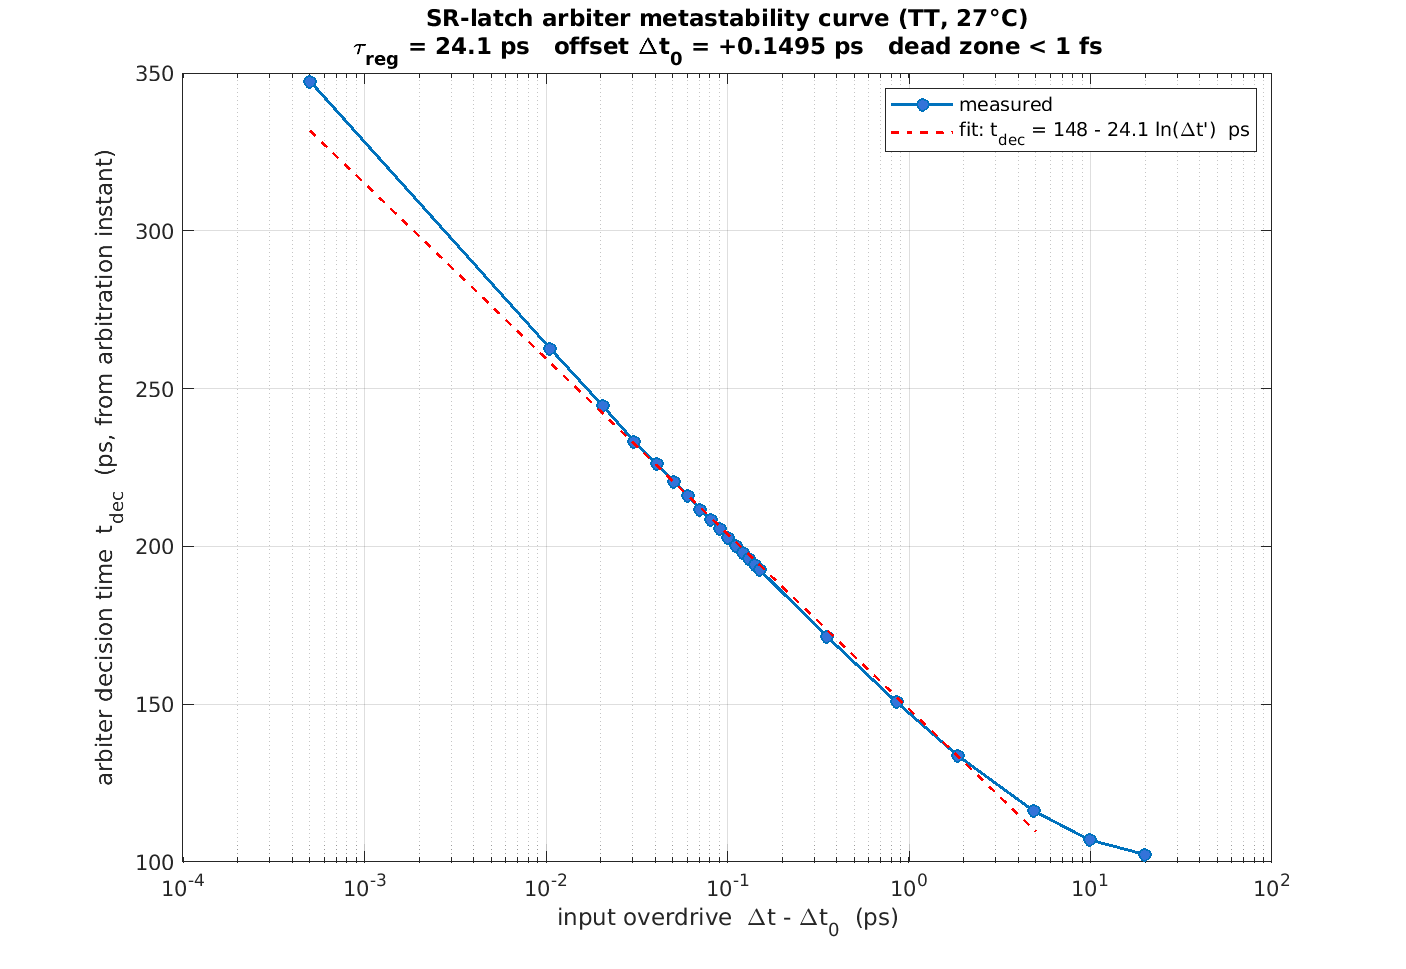
\includegraphics[width=\textwidth]{figures/metastability_curve.png}
  \caption{Decision time vs input overdrive.}
  \label{fig:metacurve}
\end{subfigure}\hfill
\begin{subfigure}[t]{0.49\textwidth}
  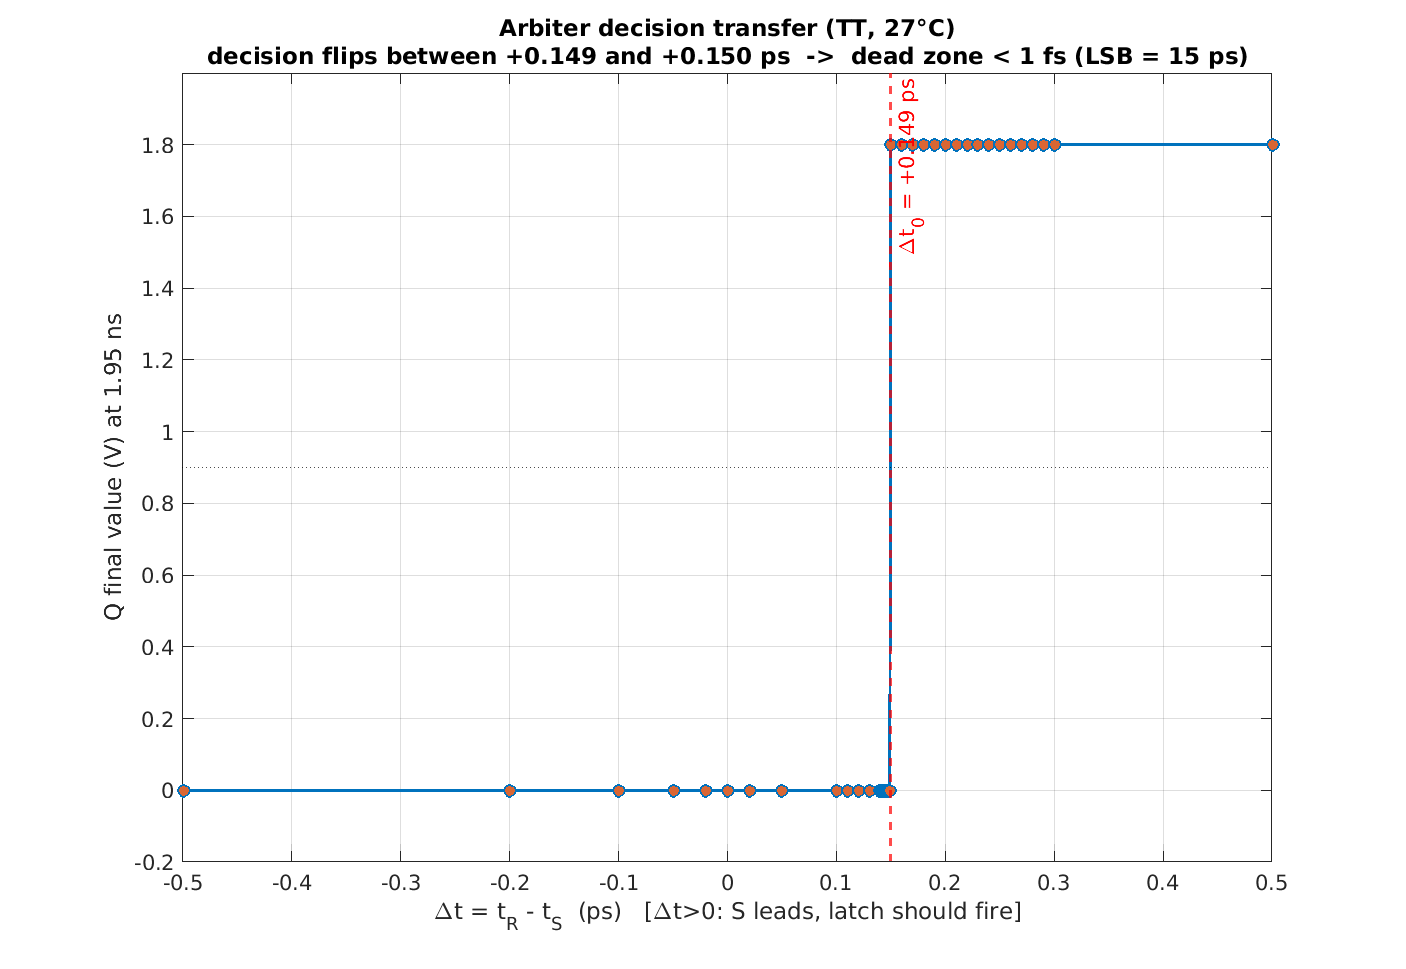
\includegraphics[width=\textwidth]{figures/deadzone_transfer.png}
  \caption{Final output vs $\dt$: the decision flips between adjacent
  \SI{1}{\femto\second} grid points.}
  \label{fig:deadzone}
\end{subfigure}
\caption{SR-latch arbiter characterization (TT, \SI{27}{\celsius},
\SI{5}{\femto\farad} loads), 49 simulations in three nested sweeps.}
\label{fig:meta}
\end{figure}

The smallest resolvable interval of the converter is set by the arbiter, so we
characterized it down to \SI{0.5}{\femto\second} of input overdrive
(Fig.~\ref{fig:meta}). The arbitration offset is
$\dt_0 = +149.5\pm\SI{0.5}{\femto\second}$, about 1\% of one LSB. The decision
time follows the classic regeneration law
$t_{dec} = t_{cq} + \tau_{reg}\ln(1/\dt')$ over three and a half decades with
$\tau_{reg}=\SI{24.1}{\pico\second}$ and a large-overdrive clk-to-Q of
\SI{102}{\pico\second}; the worst observed decision time is
\SI{347.5}{\pico\second} at \SI{0.5}{\femto\second} overdrive, still far
inside the conversion window. No ambiguous final value was observed anywhere
on the \SI{1}{\femto\second} grid, bounding the dead zone below
\SI{1}{\femto\second}, four orders of magnitude under the LSB. The bound is
grid-limited and noiseless (a Monte-Carlo analysis would widen it), which
still leaves orders of magnitude of margin.

\subsection{Measured comparison with a 1-D Vernier}
\label{sec:1dvs2d}

\begin{figure}[htb]
\centering
\begin{subfigure}[t]{0.49\textwidth}
  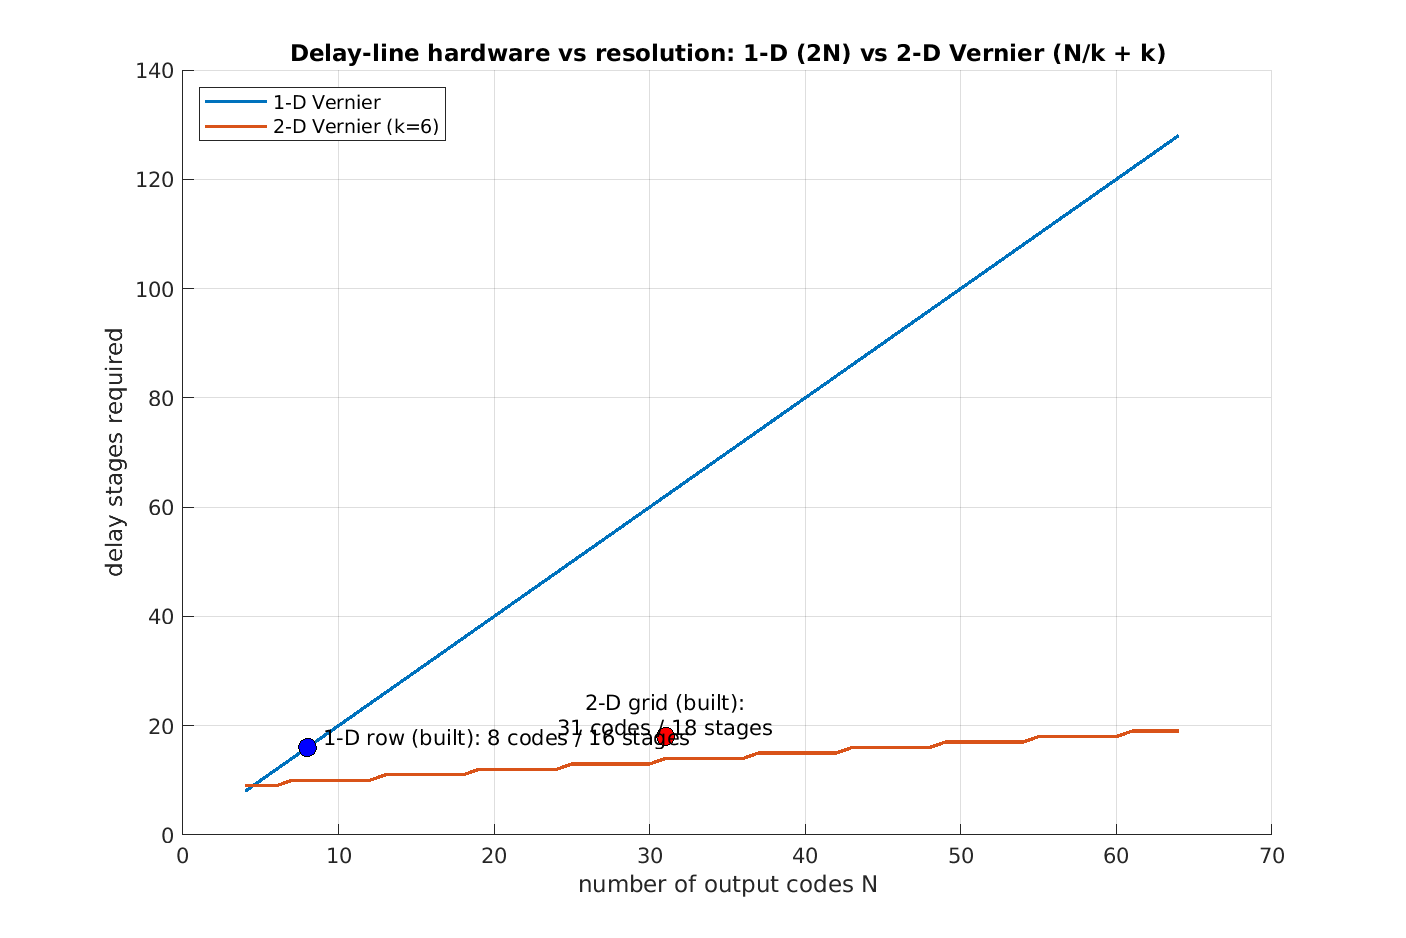
\includegraphics[width=\textwidth]{figures/scaling_1d_vs_2d.png}
  \caption{Delay stages required vs code count, with both built designs
  marked.}
  \label{fig:scaling}
\end{subfigure}\hfill
\begin{subfigure}[t]{0.49\textwidth}
  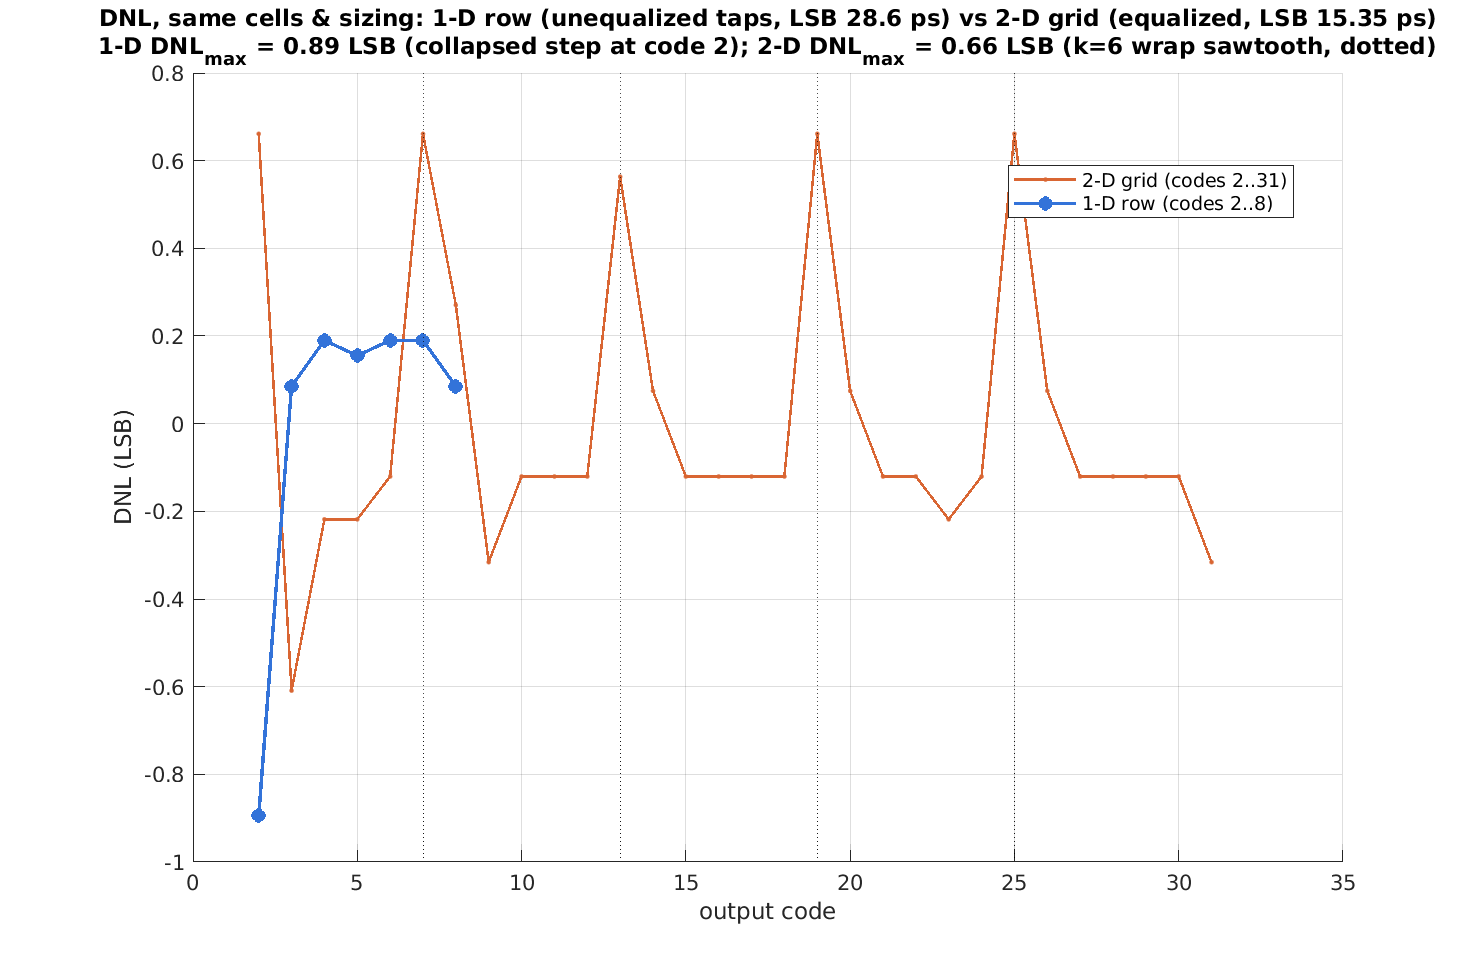
\includegraphics[width=\textwidth]{figures/dnl_1d_vs_2d.png}
  \caption{DNL, 1-D row vs 2-D core, same cells.}
  \label{fig:dnl1d2d}
\end{subfigure}
\caption{Architecture comparison from identical cells (TT).}
\label{fig:1dvs2d}
\end{figure}

To separate the architecture from the circuit design we assembled an 8-code
1-D Vernier row (\texttt{vernier2d/vernier1d\_row}) from the same delay and
latch cells, with trim banks hardwired on and, deliberately, no fan-out
equalization. Table~\ref{tab:1dvs2d} compares the measurements. The row
resolves \SI{28.6}{\pico\second} where the stage-level prediction was
\SI{16.6}{\pico\second}, confirming the loading analysis of
Section~\ref{sec:loading}, and the 2-D core is about twice as area-efficient
per code at comparable energy. Scaled to the full 31 codes, the row would
need $3.4\times$ the delay stages, $1.9\times$ the width and
\SI{3.3}{\nano\second} of full-scale latency against \SI{0.9}{\nano\second}
for the grid.

\begin{table}[H]
\centering
\small
\caption{Measured 1-D row vs 2-D core, identical cells (TT,
\SI{27}{\celsius}).}
\label{tab:1dvs2d}
\begin{tabular}{l c c}
\toprule
 & \textbf{1-D row (built)} & \textbf{2-D core (built)} \\
\midrule
Codes & 8 & 31 \\
LSB & \SI{28.6}{\pico\second} & \SI{15.35}{\pico\second} \\
DNL$_{\max}$ & 0.89 LSB & 0.66 LSB \\
Delay stages & 16 & 18 \\
$\sumw$ per code & \SI{81.4}{\micro\meter} & \SI{42.1}{\micro\meter} \\
Energy per code & \SI{0.33}{\pico\joule} & \SI{0.38}{\pico\joule} \\
Full-scale latency (31 codes) & \SI{3.3}{\nano\second} & \SI{0.9}{\nano\second} \\
\bottomrule
\end{tabular}
\end{table}

\section{Conclusion}
\label{sec:conclusion}

We built and verified a 5-bit two-dimensional Vernier TDC in TSMC
\SI{180}{\nano\meter} BCD that meets every project requirement with margin.
With a single fixed trim setting the converter resolves
\SIrange{13.1}{18.2}{\pico\second} across all five process corners with no
missing codes (worst DNL \num{0.90} LSB); per-corner MOSCAP trimming
re-centers the LSB to \SIrange{15.0}{15.85}{\pico\second}, a six times tighter
spread, without changing a single device. The core consumes
\SI{11.7}{\pico\joule} per conversion in the typical corner at a figure of
merit of \SI{0.50}{\pico\joule} per step, within a total transistor width of
\SI{1305.6}{\micro\meter}. The arbiter contributes an offset of 1\% of an LSB
and a dead zone bounded below \SI{1}{\femto\second}, so the resolution is set
by the architecture, not by the decision element.

The evidence supports three conclusions beyond the headline numbers. First,
delay-cell sizing for Vernier grids must be done against the in-grid load;
the measured 1-D row shows the LSB doubling when tap loading is ignored.
Second, fan-out equalization with dummy latches is what makes the grid
thresholds usable; it costs 29 inactive cells and buys corner-independent
linearity. Third, the bijective $k=6$ mapping removes all combining logic,
and the only systematic linearity signature left, the period-6 wrap sawtooth,
is architectural and identical in every corner.

\paragraph{Recommendations.}
Three extensions would add the most value. A DLL-style background loop could
set the trim codes automatically, replacing the static calibration table. A
voltage-to-time front end would let the TDC quantize voltages directly,
addressing the course bonus. And a targeted capacitive correction at the four
column-wrap codes could suppress the period-6 DNL pattern that calibration
cannot reach. Layout and extracted re-simulation remain the natural next step
toward silicon; the schematic-level margins reported here (\SI{4}{\pico\second}
on resolution, four orders of magnitude on the dead zone) leave realistic room
for parasitic degradation.


% ===================== References =====================
\begin{thebibliography}{9}
\small

\bibitem{liscidini2009}
A.~Liscidini, L.~Vercesi, and R.~Castello,
``Time to digital converter based on a 2-dimensions Vernier architecture,''
in \emph{Proc. IEEE Custom Integrated Circuits Conference (CICC)}, 2009, pp.~45--48.

\bibitem{vercesi2010}
L.~Vercesi, A.~Liscidini, and R.~Castello,
``Two-dimensions Vernier time-to-digital converter,''
\emph{IEEE J. Solid-State Circuits}, vol.~45, no.~8, pp.~1504--1512, Aug. 2010.

\bibitem{dudek2000}
P.~Dudek, S.~Szczepa\'nski, and J.~V. Hatfield,
``A high-resolution CMOS time-to-digital converter utilizing a Vernier delay line,''
\emph{IEEE J. Solid-State Circuits}, vol.~35, no.~2, pp.~240--247, Feb. 2000.

\bibitem{staszewski2005}
R.~B. Staszewski, S.~Vemulapalli, P.~Vallur, J.~Wallberg, and P.~T. Balsara,
``Time-to-digital converter for RF frequency synthesis in 90 nm CMOS,''
in \emph{Proc. IEEE Radio Frequency Integrated Circuits (RFIC) Symposium}, 2005,
pp.~473--476.

\bibitem{yu2010}
J.~Yu, F.~F. Dai, and R.~C. Jaeger,
``A 12-bit Vernier ring time-to-digital converter in 0.13~$\mu$m CMOS technology,''
\emph{IEEE J. Solid-State Circuits}, vol.~45, no.~4, pp.~830--842, Apr. 2010.

\bibitem{henzler2008}
S.~Henzler \emph{et al.},
``A local passive time interpolation concept for variation-tolerant high-resolution
time-to-digital conversion,''
\emph{IEEE J. Solid-State Circuits}, vol.~43, no.~7, pp.~1666--1676, Jul. 2008.

\bibitem{henzlerbook}
S.~Henzler, \emph{Time-to-Digital Converters},
Springer Series in Advanced Microelectronics, vol.~29, Springer, 2010.

\bibitem{ee4615tb}
EE4615 course staff, \emph{EE4615 Testbench Instructions}, Delft University of
Technology, Apr. 2026.

\bibitem{ee4615corner}
EE4615 course staff, \emph{EE4615 Corner Analysis Manual}, Delft University of
Technology, Apr. 2026.

\end{thebibliography}

\appendix
\section{Per-corner trim configurations}
\label{app:trim}

Trimming sets the six trim-bank gates (\texttt{trim<0:2>} of each line) to
\SI{0}{\volt} or \SI{1.8}{\volt}. Table~\ref{tab:trim} lists the winning
configuration per corner from the exhaustive 64-point probe, together with the
stage delays it produces. The FS optimum coincides with the default setting.

\begin{table}[H]
\centering
\small
\caption{Trim codes per corner and the stage delays they produce. In the code
$b_2 b_1 b_0$, bank $i$ is engaged when $b_i = 1$ (gate at \SI{1.8}{\volt});
bank weights ($b_0/b_1/b_2$) are $2/20/21$ fingers on the $\ttau{1}$ cell and
$2/14/18$ on the $\ttau{2}$ cell.}
\label{tab:trim}
\begin{tabular}{l c c S[table-format=2.1] S[table-format=2.1] S[table-format=2.2]}
\toprule
\textbf{Corner} & {$\ttau{1}$ code} & {$\ttau{2}$ code} &
{$\ttau{1}$ (\si{\pico\second})} & {$\ttau{2}$ (\si{\pico\second})} & {$\tlsb$ (\si{\pico\second})} \\
\midrule
TT & 010 & 010 & 88.5 & 73.4 & 15.04 \\
SS & 001 & 001 & 93.0 & 78.0 & 14.91 \\
FF & 111 & 111 & 90.5 & 75.6 & 14.97 \\
SF & 100 & 011 & 89.8 & 74.7 & 15.07 \\
FS & 011 & 011 & 92.6 & 77.6 & 15.01 \\
\bottomrule
\end{tabular}
\end{table}

The stage-level probe slightly underestimates the staircase LSB (SS:
\SI{14.91}{\pico\second} probe vs \SI{15.85}{\pico\second} measured) because
grid loading beyond the first stage adds a corner-dependent few percent. This
is why every configuration was re-validated with a full staircase sweep.

\section{Transistor-width budget}
\label{app:sigmaw}

Table~\ref{tab:sigmaw} breaks the netlist-extracted $\sumw$ of
\texttt{tdc\_core} down per cell, summed over all instantiations.

\begin{table}[H]
\centering
\small
\caption{$\sumw$ breakdown of the core (Spectre netlist, TT trim setting). MOSCAPs identified by drain, source and bulk tied together. The
grand total is quoted as \SI{1305.6}{\micro\meter} in the text.}
\label{tab:sigmaw}
\begin{tabular}{l S[table-format=4.2]}
\toprule
\textbf{Group} & {$\sumw$ (\si{\micro\meter})} \\
\midrule
\texttt{delay\_tau1} (11 inst.) & 450.89 \\
\texttt{delay\_tau2} (7 inst.) & 207.34 \\
\texttt{nand} (latch gates) & 211.20 \\
\texttt{srlatch} (reset devices) & 120.00 \\
\texttt{Inv} (latch output buffers) & 114.84 \\
\texttt{Inv\_20x} & 92.40 \\
\texttt{Inv\_80x} & 52.80 \\
\texttt{Inv\_40x} & 26.40 \\
\texttt{Inv\_10x} & 19.80 \\
\texttt{Inv\_5x} & 9.90 \\
\midrule
Active total (1120 devices) & 1078.32 \\
MOSCAP trim banks (65 devices) & 227.25 \\
\textbf{Grand total (1185 devices)} & \textbf{1305.57} \\
\bottomrule
\end{tabular}
\end{table}

\section{Simulation inventory}
\label{app:sims}

All results are reproducible from the OCEAN scripts submitted with the design.

\begin{itemize}
  \item \textbf{Corner campaign} (\texttt{tdc\_corners\_all.ocn}): five
  corners, \SI{1.5}{\pico\second} delay step, 1670 transients; produces the
  transition tables behind Figs.~\ref{fig:staircase}--\ref{fig:linearity} and
  Table~\ref{tab:corners}.
  \item \textbf{Trim probe} (\texttt{tune\_probe.ocn}): 64 trim
  configurations $\times$ 5 corners, 320 transients; produces
  Fig.~\ref{fig:calrange} and Table~\ref{tab:trim}.
  \item \textbf{Trimmed campaign} (\texttt{tdc\_tuned\_all.ocn}): repeats
  the corner campaign with per-corner trim codes; produces
  Fig.~\ref{fig:lsbtuned}.
  \item \textbf{Metastability} (\texttt{meta\_sweep\_\{coarse,fine,ultra\}.ocn}):
  three nested sweeps, 49 transients, overdrive resolved to
  \SI{0.5}{\femto\second}; produces Fig.~\ref{fig:meta}.
  \item \textbf{1-D comparison} (\texttt{v1d\_staircase\_v2.ocn},
  \texttt{v1d\_energy2.ocn}): 321-run staircase and energy measurement of the
  1-D row; produces Fig.~\ref{fig:1dvs2d} and Table~\ref{tab:1dvs2d}.
\end{itemize}


\end{document}
